\documentclass[10pt,a4paper]{amsart}
\usepackage[margin=19mm]{geometry}
\usepackage{amsmath,amssymb,mathtools}
\usepackage[scr=rsfs,cal=euler]{mathalfa}
\usepackage{xfrac}
\usepackage[unicode,hidelinks,bookmarks=false]{hyperref}
\newcommand{\ie}{i.e.\ }
\newcommand{\cf}{cf.\ }
\newcommand{\resp}{respectively\ }
\newcommand{\Subsection}{\subsection}
\providecommand{\nobreakdash}{\nobreak\hbox{-}}
\setlength{\emergencystretch}{2em}
\multlinegap0pt
\usepackage{tikz}
\usepackage{float}
\usepackage{amssymb}
\usepackage{mathtools}
\usepackage{xcolor}
\newtheorem{defn}{Definition}
\newtheorem{lemma}{Lemma}
\newtheorem{claim}{Claim}
\usepackage{cleveref}
\crefname{defn}{Definition}{Definitions}
\crefname{lemma}{Lemma}{Lemmas}
\crefname{claim}{Claim}{Claims}
\newcommand{\PP}{\mathcal{P}}
\newcommand{\RR}{\mathbb{R}}
\newcommand{\define}[1]{\textbf{#1}}
\newcommand{\init}{\mathfrak{i}}
\newcommand{\norm}[1]{\|{#1}\|}
\newcommand{\pos}{\operatorname{pos}}
\newcommand{\supp}{\textnormal{supp}}
\newcommand{\ter}{\mathfrak{t}}
\newcommand{\val}{\operatorname{val}}
\title{A general framework for quasi-isometries in symbolic dynamics beyond groups}
\author{Sebasti\'an Barbieri, Nicol\'as Bitar}
\date{Source: arXiv:2504.05194v2 (CC BY 4.0)}
\begin{document}
\maketitle

\noindent\emph{Source and licence.} A general framework for quasi-isometries in symbolic dynamics beyond groups. Version arXiv:2504.05194v2 (CC BY 4.0), distributed by arXiv under the Creative Commons Attribution 4.0 International licence, http://creativecommons.org/licenses/by/4.0/, as recorded in the arXiv licence metadata for this exact version and shown on the abstract page https://arxiv.org/abs/2504.05194v2. Full licence notice: \texttt{licenses/arxiv-2504.05194-CC-BY-4.0.txt}.\par\smallskip

\noindent\textit{Editorial scope.} Counted unit: the article's claim claim:forma\_canonica (source0.tex lines 1591--1593). The article's complete original proof of it is delivered with it (source0.tex lines 1595--1676, one \texttt{proof} environment of 82 lines). No mathematics is written, repaired or re-derived: the statement and the proof are the article's own lines, in the article's own notation, and no retained line is substituted or re-flowed.  Retained uncounted as the source-local context the proof needs: lines 1451--1453; lines 1471--1478.  Nothing was omitted from any retained span, so the package carries no omission record.  No retained line contains a citation, so the wrapper carries no bibliography and no bibliography entry.  The retained lines contain the article's own diagram code, which the wrapper typesets with the standard tikz packages; no image file is delivered and the package declares no asset dependency.  Editorial formatting only, in addition: an AMS \texttt{amsart} preamble that restates the article's own declarations and macros used by the retained lines, namely the environments \texttt{defn}, \texttt{lemma}, \texttt{claim} on separate counters, together with the standard packages those lines need.  The retained environments print in this document as Definition 1, Lemma 1, Claim 1 in order of appearance, whereas the article prints the same items with the numbering of its own full document.  The complete native source of the article as distributed in the arXiv e-print for this exact version is bundled unchanged as \texttt{sources/176125/source0.tex}.
\begin{defn}\label{def:patchblueprint}
    Fix positive integers $K,L$. The \define{patch blueprint} of a set of punctured tiles $\PP$ with FLC is the finitely presented blueprint $\Gamma(\PP,K,L) = (M,S,\init,\ter,R)$ where $M, S, \init,\ter$ and $R$, are given as above.
\end{defn}

\begin{lemma}[Interpolation]
\label{lem:sausage}
    Let $T$ be a partial tiling by translations of punctured tiles in $\PP$ whose support contains a convex set $C\subset \RR^d$. For any distinct $x,y \in C$ if we take $n = \lceil  \rho^{-1}\norm{y-x}\rceil$, there exists a sequence of tiles $t_0,\dots, t_{n}  \in T$ such that:
    \begin{enumerate}
        \item For every $k \in \{0,\dots,n\}$ we have $\norm{\pos(t_k)- (x +\frac{k}{n}(y-x))}\leq \rho$,
        \item For every $k \in \{1,\dots,n\}$ we have $\norm{\pos(t_k)-\pos(t_{k-1})}\leq 3\rho$.
        \end{enumerate}
\end{lemma}

    \begin{claim}\label{claim:forma_canonica}
        Let $w\in \mathcal{R}(n+1)$ be a nonempty word. There exists $u \in \mathcal{R}(n)$ and $s \in S$ such that $us \in \supp(\varphi)$ and $us$ is $\Gamma$-equivalent to $w$. In particular $\varphi(us)+\val(us) = \varphi(w)+\val(w)$.
    \end{claim}

    \begin{proof}
        Write $w=s_1\dots s_k$ with each $s_i \in S$ and let $w_i = s_1\dots s_i$ and $w_0 = \varepsilon$. If for every $i\in \{1,\dots,k-1\}$ we have $\norm{\val(w_i)}\leq n\rho$, then we can just take $u = w_{k-1}$ and $s = s_k$. Otherwise, let $j$ be the smallest positive integer such that $\norm{\val(w_j)}>n \rho$.

        Take $y,z \in \RR^d$ as follows:
        \begin{align*}
            y & = \begin{cases}
            (n-1)\rho\frac{\val(w_{j-1})}{\norm{\val(w_{j-1})}} & \mbox{if } \norm{\val(w_{j-1})} > 0,\\
            0 & \mbox{otherwise}.
        \end{cases}\\
        z & = \begin{cases}
            (n-1)\rho\frac{\val(w_{j+1})}{\norm{\val(w_{j+1})}} & \mbox{if } \norm{\val(w_{j+1})} > 0,\\
            0 & \mbox{otherwise}.
        \end{cases} 
        \end{align*}
        As $w\in \mathcal{R}(n+1)$, we have that both $\norm{\val(w_{j-1})}$ and $\norm{\val(w_{j+1})}$ are at most $(n+1)\rho$. Moreover, as $\norm{\val(w_j)}>n \rho$, we have that $\norm{\val(w_{j-1})}$ and $\norm{\val(w_{j+1})}$ are at least $(n-3)\rho$ and thus we deduce that both values belong to the interval $\bigl( (n-3)\rho, (n+1)\rho)\bigr)$.
        
        It follows that by construction of $y$ and $z$ we have that both $\norm{y-\val(w_{j-1})} \leq 2\rho$ and $\norm{\val(w_{j+1})-z}\leq 2\rho$. From this and the fact $\norm{\val(w_{j-1})- \val(w_{j+1})}\leq 6\rho$ we obtain that
        \[ \norm{y-z} \leq \norm{y-\val(w_{j-1})} + \norm{\val(w_{j-1})- \val(w_{j+1})} + \norm{ \val(w_{j+1})-z} \leq 10\rho.   \]

         \begin{figure}[h!]
        \centering
        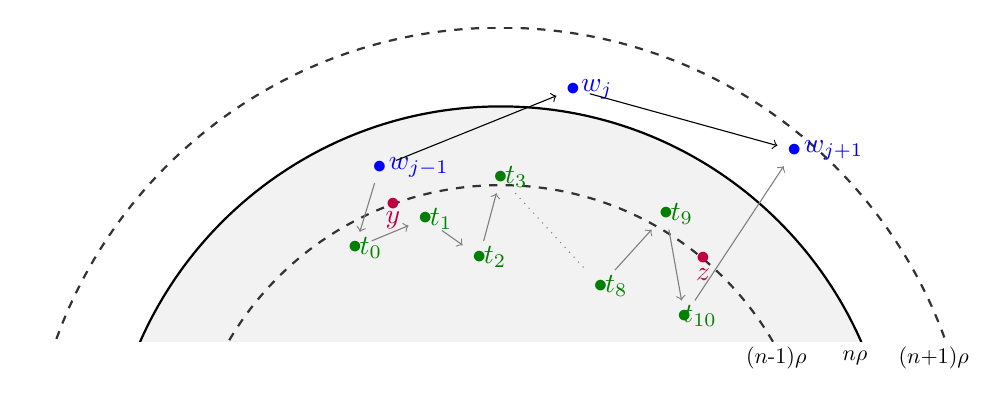
\begin{tikzpicture}
        {\clip (-6,1.5) rectangle (6,6);
            \draw[thick, fill = black!05] (0,0) circle (5);
            \draw[thick, dashed, color=black!80] (0,0) circle (6);
            \draw[thick, dashed, color=black!80] (0,0) circle (4);
             \node[blue] (A) at ({4.5*cos(110)},{4.5*sin(110)}){$\bullet$};
             \node[blue] at ({0.5+4.5*cos(110)},{4.5*sin(110)}){$w_{j-1}$};
             \node[blue] (B) at ({5.3*cos(80)},{5.3*sin(80)}){$\bullet$};
             \node[blue] at ({0.3+5.3*cos(80)},{5.3*sin(80)}){$w_{j}$};
             \node[blue] (C) at ({5.8*cos(50)},{5.8*sin(50)}){$\bullet$};
             \node[blue] at ({0.5+5.8*cos(50)},{5.8*sin(50)}){$w_{j+1}$};
             \node[purple] (BB) at ({4*cos(110)},{4*sin(110)}){$\bullet$};
             \node[purple] at ({4*cos(110)},{4*sin(110)-0.2}){$y$};
             \node[purple] (CC) at ({4*cos(50)},{4*sin(50)}){$\bullet$};
             \node[purple] at ({4*cos(50)},{4*sin(50)-0.2}){$z$};
             \node[black!50!green] (D0) at ({3.7*cos(120)},{3.7*sin(120)}){$\bullet$};
             \node[black!50!green] at ({3.7*cos(120)+0.2},{3.7*sin(120)}){$t_0$};
             \node[black!50!green] (D1) at ({3.7*cos(105)},{3.7*sin(105)}){$\bullet$};
             \node[black!50!green] at ({3.7*cos(105)+0.2},{3.7*sin(105)}){$t_1$};
             \node[black!50!green] (D2) at ({3.1*cos(95)},{3.1*sin(95)}){$\bullet$};
             \node[black!50!green] at ({3.1*cos(95)+0.2},{3.1*sin(95)}){$t_2$};
             \node[black!50!green] (D3) at ({4.1*cos(90)},{4.1*sin(90)}){$\bullet$};
             \node[black!50!green] at ({4.1*cos(90)+0.2},{4.1*sin(90)}){$t_3$};
             \node[black!50!green] (D4) at ({3*cos(65)},{3*sin(65)}){$\bullet$};
             \node[black!50!green] at ({3*cos(65)+0.2},{3*sin(65)}){$t_8$};
             \node[black!50!green] (D5) at ({4.2*cos(60)},{4.2*sin(60)}){$\bullet$};
             \node[black!50!green] at ({4.2*cos(60)+0.2},{4.2*sin(60)}){$t_9$};
             \node[black!50!green] (D6) at ({3.3*cos(45)},{3.3*sin(45)}){$\bullet$};
             \node[black!50!green] at ({3.3*cos(45)+0.2},{3.3*sin(45)}){$t_{10}$};
             \draw[color =black!50, -> ] (A) to (D0);
             \draw[color =black!50, -> ] (D0) to (D1);
             \draw[color =black!50, -> ] (D1) to (D2);
             \draw[color =black!50, -> ] (D2) to (D3);
             \draw[color =black!50, dotted ] (D3) to (D4);
             \draw[color =black!50, -> ] (D4) to (D5);
             \draw[color =black!50, -> ] (D5) to (D6);
             \draw[color =black!50, -> ] (D6) to (C);
             \draw[color =black, -> ] (A) to (B);
             \draw[color =black, -> ] (B) to (C);}
             \draw [fill = white, color=white] (-6,1.5) rectangle (6,2);
             \node at (4.5,1.8) {\scalebox{0.8}{$n\rho$}};
             \node at (5.5,1.8) {\scalebox{0.8}{$(n\text{+}1)\rho$}};
             \node at (3.5,1.8) {\scalebox{0.8}{$(n\text{-}1)\rho$}};
            
        \end{tikzpicture}
        \caption{Sketch of the proof of~\Cref{claim:forma_canonica}}
        \label{fig:proof_forma_canonica}
    \end{figure}
        
        By~\Cref{lem:sausage} applied to $y,z$ and $T_n$, we obtain that there is a sequence $t_0,\dots,t_{10}$ of tiles in $T_n$ which are at consecutive distance at most $3\rho$ and at distance $\rho$ from the interval between $y$ and $z$. For each $\ell \in \{0,\dots,10\}$ take $u_{\ell}\in \mathcal{R}(n)$ such that $t_{\ell}=t_{u_{\ell}}$, see~\Cref{fig:proof_forma_canonica} for a sketch of this construction. Consider now the tuples 
        \begin{align*}
            a_0 &  = (\varphi(w_{j-1}), \val(u_0) -\val(w_{j-1}))\\
            a_i & = (\varphi(u_{i-1}),\val(u_{i-1})-\val(u_i)) \mbox{ for } i \in \{1,\dots,10\}\\
            a_{11} & = (\varphi(u_{10}),\val(w_{j+1})-\val(u_{10})).
        \end{align*}

        Notice that each of the second coordinates gives a vector of length at most $3\rho$. Moreover, by the inductive hypothesis, all of the patches in the first coordinate match pairwise, thus $a_0,\dots,a_{11} \in S$ and  $w_{j-1}a_0\dots a_{11} \in \supp(\varphi)$.
        
        Finally, notice that if we remove the last generator, we have $w_{j-1}a_0\dots a_{10} \in \mathcal{R}(n)$. Moreover, we have \[\val(a_0\dots a_{11}) = \val(w_{j+1})-\val(w_{j-1}) =\val(s_js_{j+1}).\]
        As $|a_0\dots a_{11}| + |s_js_{j+1}|\leq L$, it follows that $(a_0,\dots, a_{11},s_js_{j+1}) \in R$ (recall the definition of $R$ before~\Cref{def:patchblueprint}), in particular, the words $w_{j-1}a_0\dots a_{11}$ and $w_{j+1}$ are $\Gamma$-equivalent. Replacing $w_{j+1}$ by $w_{j-1}a_0\dots a_{11}$, we obtain a $\Gamma$-equivalent word where the value $k-j$ has been reduced by at least $1$. We obtain the desired decomposition iterating this procedure.
    \end{proof}

\end{document}
